
% Document class: article with font size 11pt
% ---------------
\documentclass[11pt,a4paper]{report}

% Call packages
% ---------------
\usepackage{comment} %Possible to comment larger sections
%http://get-software.net/macros/latex/contrib/comment/comment.pdf
\usepackage[T1]{fontenc} %oriented to output, that is, what fonts to use for printing characters.
\usepackage[utf8]{inputenc} %allows the user to input accented characters directly from the keyboard
%Put fontenc before inputenc
\usepackage{fourier} %Better typeface
%http://mirrors.dotsrc.org/ctan/fonts/fourier-GUT/doc/latex/fourier/fourier-doc-en.pdf
\usepackage[danish]{babel}														     % Danish
\usepackage[protrusion=true,expansion=true]{microtype}				                 % Better typography
%http://www.khirevich.com/latex/microtype/
\usepackage{amsmath,amsfonts,amsthm, amssymb}							 % Math packages
\usepackage[pdftex]{graphicx} %puts to pdf and graphic
%http://www.kwasan.kyoto-u.ac.jp/solarb6/usinggraphicx.pdf
\usepackage{xcolor,colortbl}
%http://mirrors.dotsrc.org/ctan/macros/latex/contrib/xcolor/xcolor.pdf
%http://texdoc.net/texmf-dist/doc/latex/colortbl/colortbl.pdf
\usepackage{tikz} %documentation http://www.ctan.org/pkg/pgf
\usetikzlibrary{arrows,positioning} %http://tex.stackexchange.com/questions/141842/tikz-self-loops-style-question
\tikzset{
    >=stealth,
    %auto,
    %node distance=3.5cm,
    font=\scriptsize,
    empty world/.style={align=center},
    single world/.style={circle,draw,thick,align=center},
    double world/.style={double,circle,draw,thick,align=center},
    minimum size=40pt
}

%\usetikzlibrary{matrix}
\usepackage{parskip} %http://www.ctan.org/pkg/parskip
%http://tex.stackexchange.com/questions/51722/how-to-properly-code-a-tex-file-or-at-least-avoid-badness-10000
%Never use \\ but instead press "enter" twice. See second website for more info
\usepackage{natbib}
%\usepackage{tablefootnote}
%Brug H for figur lige HER!!
\usepackage{float}
%\caption{} til tabeller
\usepackage{caption}

\usepackage{pbox}

%Skal ikke bruges i slut
\usepackage[draft,danish]{fixme} %Danish latex book
%\usepackage{showkeys} %Brug kun til at holde styr på labels

%%--------------------------------
%Til at vise links i pdf filen så man kan hoppe frem og tilbage
\usepackage{hyperref}
\hypersetup{
    colorlinks,
    linkcolor={blue!35!black},
    citecolor={blue!50!black},
    urlcolor={blue!80!black}
}

\usepackage{fancyhdr} % Required for custom headers
\usepackage{lastpage} % Required to determine the last page for the footer
\usepackage{extramarks} % Required for headers and footers
\usepackage{listings} % Required for insertion of code
\usepackage{courier} % Required for the courier font
\usepackage{lipsum} % Used for inserting dummy 'Lorem ipsum' text into the template


\usepackage[top=1in, bottom=1.25in, left=1.25in, right=1.25in, footskip=0.25in]{geometry}

\linespread{1.15} % Line spacing

% Set up the header and footer
\pagestyle{fancy}
\lhead{\hmwkAuthorName} % Top left header
\chead{\hmwkClass\: \hmwkTitle} % Top center head
\rhead{\firstxmark} % Top right header
\lfoot{\lastxmark} % Bottom left footer
\cfoot{} % Bottom center footer
\rfoot{Page\ \thepage\ of\ \protect\pageref{LastPage}} % Bottom right footer
\renewcommand\headrulewidth{0.4pt} % Size of the header rule
\renewcommand\footrulewidth{0.4pt} % Size of the footer rule

\setlength\parindent{0pt} % Removes all indentation from paragraphs

%----------------------------------------------------------------------------------------
%	DOCUMENT STRUCTURE COMMANDS
%	Skip this unless you know what you're doing
%----------------------------------------------------------------------------------------

% Header and footer for when a page split occurs within a problem environment
\newcommand{\enterProblemHeader}[1]{
\nobreak\extramarks{#1}{#1 continued on next page\ldots}\nobreak
\nobreak\extramarks{#1 (continued)}{#1 continued on next page\ldots}\nobreak
}

% Header and footer for when a page split occurs between problem environments
\newcommand{\exitProblemHeader}[1]{
\nobreak\extramarks{#1 (continued)}{#1 continued on next page\ldots}\nobreak
\nobreak\extramarks{#1}{}\nobreak
}

\setcounter{secnumdepth}{0} % Removes default section numbers
\newcounter{homeworkProblemCounter} % Creates a counter to keep track of the number of problems

\newcommand{\homeworkProblemName}{}
\newenvironment{homeworkProblem}[1][Task \arabic{homeworkProblemCounter}]{ % Makes a new environment called homeworkProblem which takes 1 argument (custom name) but the default is "Problem #"
\stepcounter{homeworkProblemCounter} % Increase counter for number of problems
\renewcommand{\homeworkProblemName}{#1} % Assign \homeworkProblemName the name of the problem
\section{\homeworkProblemName} % Make a section in the document with the custom problem count
\enterProblemHeader{\homeworkProblemName} % Header and footer within the environment
}{
\exitProblemHeader{\homeworkProblemName} % Header and footer after the environment
}

\newcommand{\problemAnswer}[1]{ % Defines the problem answer command with the content as the only argument
\noindent\framebox[\columnwidth][c]{\begin{minipage}{0.98\columnwidth}#1\end{minipage}} % Makes the box around the problem answer and puts the content inside
}

\newcommand{\homeworkSectionName}{}
\newenvironment{homeworkSection}[1]{ % New environment for sections within homework problems, takes 1 argument - the name of the section
\renewcommand{\homeworkSectionName}{#1} % Assign \homeworkSectionName to the name of the section from the environment argument
\subsection{\homeworkSectionName} % Make a subsection with the custom name of the subsection
\enterProblemHeader{\homeworkProblemName\ [\homeworkSectionName]} % Header and footer within the environment
}{
\enterProblemHeader{\homeworkProblemName} % Header and footer after the environment
}

%----------------------------------------------------------------------------------------
%	NAME AND CLASS SECTION
%----------------------------------------------------------------------------------------

\newcommand{\hmwkTitle}{Assignment\ \#4} % Assignment title
\newcommand{\hmwkDueDate}{Sunday,\ January\ 10,\ 2016} % Due date
\newcommand{\hmwkClass}{Compilers} % Course/class
\newcommand{\hmwkClassTime}{Task 2 and as much as possible Task3} % Class/lecture time
\newcommand{\hmwkClassInstructor}{Resubmit:} % Teacher/lecturer
\newcommand{\hmwkAuthorName}{Mirza Hasanbasic} % Your name

%----------------------------------------------------------------------------------------
%	TITLE PAGE
%----------------------------------------------------------------------------------------

\title{
\vspace{2in}
\textmd{\textbf{\hmwkClass:\ \hmwkTitle}}\\
\normalsize\vspace{0.1in}\small{Due\ on\ \hmwkDueDate}\\
\vspace{0.1in}\large{\textit{\hmwkClassInstructor\ \hmwkClassTime}}
\vspace{3in}
}

\author{\textbf{\hmwkAuthorName}}
\date{} % Insert date here if you want it to appear below your name


%----------------------------------------------------------------------------------------
%	MATH
%----------------------------------------------------------------------------------------
%\newcommand{\Real}{\mathbb R}
%\newcommand{\Complex}{\mathbb C}
%\newcommand{\Field}{\mathbb F}
%\newcommand{\RPlus}{[0,\infty)}
%%
%\newcommand{\norm}[1]{\left\Vert#1\right\Vert}
%\newcommand{\essnorm}[1]{\norm{#1}_{\text{\rm\normalshape ess}}}
%\newcommand{\abs}[1]{\left\vert#1\right\vert}
%\newcommand{\set}[1]{\left\{#1\right\}}
%\newcommand{\seq}[1]{\left<#1\right>}
%\newcommand{\eps}{\varepsilon}
%\newcommand{\To}{\longrightarrow}
%\newcommand{\RE}{\operatorname{Re}}
%\newcommand{\IM}{\operatorname{Im}}
%\newcommand{\Poly}{{\cal{P}}(E)}
%\newcommand{\EssD}{{\cal{D}}}
%% THEOREMS ----------------------------------------------------------------
%\theoremstyle{plain}
%\newtheorem{thm}{Theorem}[section]
%\newtheorem{cor}[thm]{Corollary}
%\newtheorem{lem}[thm]{Lemma}
%\newtheorem{prop}[thm]{Proposition}
%%
%\theoremstyle{definition}
%\newtheorem{defn}{Definition}[section]
%%
%\theoremstyle{remark}
%\newtheorem{rem}{Remark}[section]
%%
%\numberwithin{equation}{section}
%\renewcommand{\theequation}{\thesection.\arabic{equation}}

\usepackage{listings}
\lstset{
  frame=single,
  numbers=left,
  mathescape=false,
  literate={->}{$\rightarrow$}{2}
           {ε}{$\varepsilon$}{1}
           {=>}{$\Rightarrow$}{2}
}

\begin{document}

\maketitle

%----------------------------------------------------------------------------------------
%	TABLE OF CONTENTS
%----------------------------------------------------------------------------------------

%\setcounter{tocdepth}{1} % Uncomment this line if you don't want subsections listed in the ToC

\newpage
\tableofcontents
\newpage

%----------------------------------------------------------------------------------------
%	PROBLEM 1
%----------------------------------------------------------------------------------------

% To have just one problem per page, simply put a \clearpage after each problem


\begin{homeworkProblem}

Nogen veje der er acceptable ville være

\begin{table}[H]
  \centering
  \begin{tabular}{|c|}
    \hline
    % after \\: \hline or \cline{col1-col2} \cline{col3-col4} ...
    a \\
    ab \\
    abb \\
    b \\
    bab \\
    baab \\
    \hline
  \end{tabular}
\end{table}

Nu kigger på hvor vi kan komme fra et punkt til et andet i de forskellige states, dette ses i tabellen nedenunder

\begin{table}[H]
  \centering
  \begin{tabular}{|c|c|c|c|}
    \hline
    % after \\: \hline or \cline{col1-col2} \cline{col3-col4} ...
     & a & b & $\epsilon^{*}$ \\ \hline
    1 & 3 & 5 & 1,2,4 \\ \hline
    2 & 3 & - & 2 \\ \hline
    3 & - & 3 & 3,6 \\ \hline
    4 & 4 & 5 & 4 \\ \hline
    5 & - & - & 4,5,6 \\ \hline
    6 & - & - & 6 \\ \hline
  \end{tabular}
  \caption{"1" er start state, "6" er ending state. Veje for en state fra et punkt til et andet. Hvor $\epsilon^{*}$ betyder nul eller flere. }
\end{table}

Da, vi har epsilons, skal vi, skal vi kigge på hvad der sker hvis vi er i en bestemt state og hvis vi derved følger en vej, hvad der sker hvis jeg følger en eller flere veje.

\begin{table}[H]
  \centering
  \begin{tabular}{|c|c|c|c|}
    \hline
    % after \\: \hline or \cline{col1-col2} \cline{col3-col4} ...
     & a$\epsilon^{*}$ & b$\epsilon^{*}$ \\
    1 & 3 ,6 & 4,5,6 \\
    3,6 & - & 3,6 \\
    4,5,6 & 4 & 4,5,6 \\
    4 & 4 & 4,5,6 \\
    \hline
  \end{tabular}
  \caption{"1" er start state, hvor "3,6" og "4,5,6" er ending state.}
\end{table}

\begin{figure}[H]
\centering
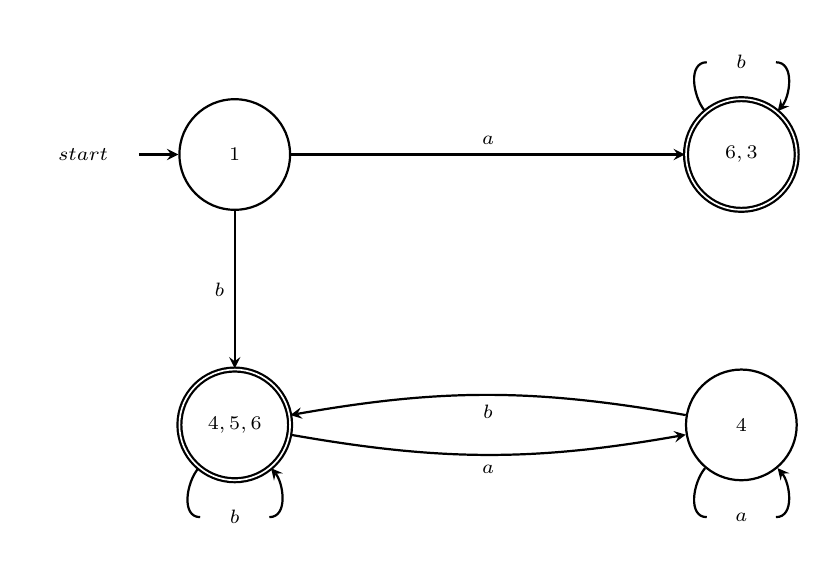
\begin{tikzpicture}
    \node[single world] (1) {$1$};
    \node[empty world] (start) [left = 0.5cm of 1] {$start$};
    \node[double world] (2) [right = 5cm of 1] {$6,3$};
    \node[above = .1ex of 2, inner sep = 0pt, outer sep = 0pt, minimum size = 25pt] (2a) {$b$};
    \node[double world] (3) [below = 2cm of 1] {$4,5,6$};
    \node[below = .1ex of 3, inner sep = 0pt, outer sep = 0pt, minimum size = 25pt] (3a) {$b$};
    \node[single world] (4) [right = 5cm of 3] {$4$};
    \node[below = .1ex of 4, inner sep = 0pt, outer sep = 0pt, minimum size = 25pt] (4a) {$a$};
    \path[]
        (2) edge [in=180, out=130, thick] (2a)
        (2a) edge [->,in=50, out=0,thick] (2)
        (3) edge [in=180, out=230, thick] (3a)
        (3a) edge [->,in=310, out=0,thick] (3)
        (4) edge [in=180, out=230, thick] (4a)
        (4a) edge [->,in=310, out=0,thick] (4)
        (start) [->, thick] edge node [] {$$} (1)
        (1) [->, thick] edge node [above, minimum size=0pt] {$a$} (2)
        (1) [->, thick] edge node [left, minimum size=0pt] {$b$} (3)
        (3) [->, thick, bend right=10] edge node [below, minimum size=0pt] {$a$} (4)
        (3) [<-, thick, bend left=10] edge node [below, minimum size=0pt] {$b$} (4)
        ;
\end{tikzpicture}
\caption{DFA repræsentationen}
\end{figure}

\end{homeworkProblem}

\begin{homeworkProblem}

Først oprettes en tabel, for at kunne se hvilke states der er forbundet. Hvor der står $3^{*}$, betyder blot at det er ending state.

\begin{figure}[H]
  \centering
  \begin{tabular}{|c|c|c|}
    \hline
    % after \\: \hline or \cline{col1-col2} \cline{col3-col4} ...
     & 0 & 1 \\ \hline
    1 & 2 & 6 \\ \hline
    2 & 7 & 3$^{*}$ \\ \hline
    3$^{*}$ & 1 & 3$^{*}$ \\ \hline
    4 & 3$^{*}$ & 7 \\ \hline
    5 & 8 & 6 \\ \hline
    6 & 3$^{*}$ & 7 \\ \hline
    7 & 7 & 5 \\ \hline
    8 & 7 & 3$^{*}$ \\ \hline
  \end{tabular}
\end{figure}

Nu sammenlignes der for hvilke indgange der kommer i andre grupper. Mange sammenligner $(q_i,q_j)$ mod hinanden og ser om de er i samme eller anden gruppe iterativt. Vi starter med 0-equal, hvor ending state vil være G2 og alle andre vil være G1.

\begin{figure}[H]
  \centering
  \begin{tabular}{|c|c|c|c|c|c|}
    \hline
    % after \\: \hline or \cline{col1-col2} \cline{col3-col4} ...
            & G1 & G2 & G3 & G4 & G5 \\ \hline
    0-equal & 1,2,4,5,6,7,8 & 3 &  &  &  \\ \hline
    1-equal & 1,5,7 & 3 & 2,8 & 4,6 &  \\ \hline
    2-equal & 1,5 & 3 & 2,8 & 4,6 & 7 \\ \hline
    3-equal & 1,5 & 3 & 2,8 & 4,6 & 7 \\ \hline
  \end{tabular}
\end{figure}

Altså er DFA minimeret og ser ud som følger

\textcolor[rgb]{0.76,0.00,0.02}{\textbf{FIX:}}

\begin{figure}[H]
\centering
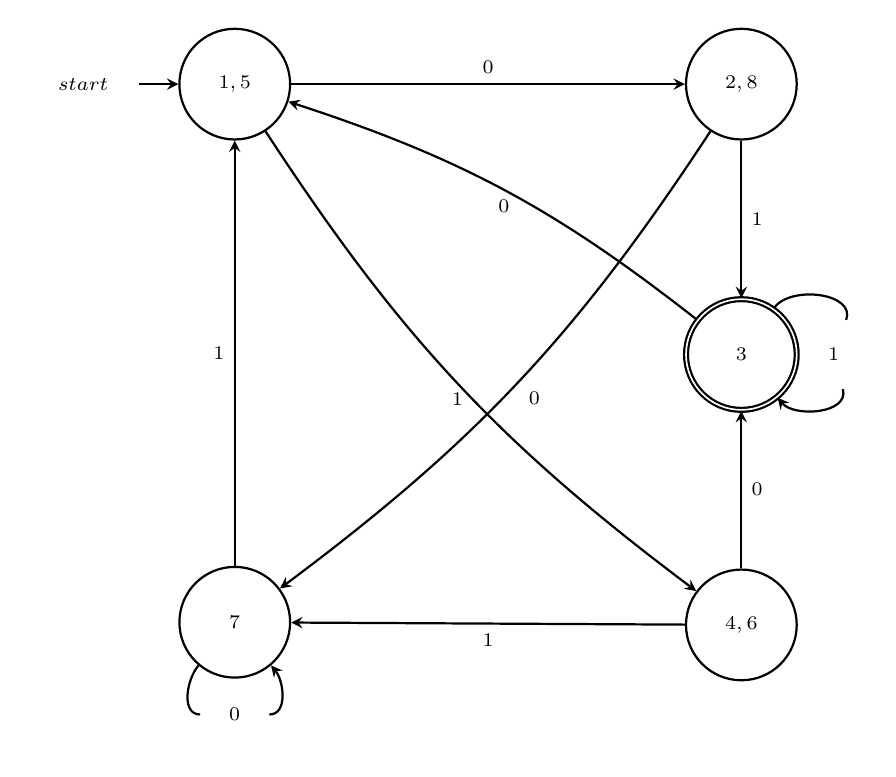
\begin{tikzpicture}
    \node[single world] (1) {$1,5$};
    \node[empty world] (start) [left = 0.5cm of 1] {$start$};
    \node[single world] (2) [below = 5.4cm of 1] {$7$};
    \node[below = .1ex of 2, inner sep = 0pt, outer sep = 0pt, minimum size = 25pt] (2a) {$0$};
    \node[single world] (3) [right = 5cm of 1] {$2,8$};
    \node[double world] (4) [below = 2cm of 3] {$3$};
    \node[right = .1ex of 4, inner sep = 0pt, outer sep = 0pt, minimum size = 25pt] (4a) {$1$};
    \node[single world] (5) [below = 2cm of 4] {$4,6$};
    \path[]
        (2) edge [in=180, out=230, thick] (2a)
        (2a) edge [->,in=310, out=0,thick] (2)
        (4) edge [in=70, out=55, thick] (4a)
        (4a) edge [->,in=310, out=285,thick] (4)
        (start) [->, thick] edge node [] {$$} (1)
        (2) [->, thick] edge node [left, minimum size=0pt] {$1$} (1)
        (1) [->, thick] edge node [above, minimum size=0pt] {$0$} (3)
        (3) [->, thick] edge node [right, minimum size=0pt] {$1$} (4)
        (5) [->, thick] edge node [right, minimum size=0pt] {$0$} (4)
        (5) [->, thick] edge node [below , minimum size=0pt] {$1$} (2)
        (1) [->, thick, bend right=10] edge node [below, minimum size=0pt] {$1$} (5)
        (3) [->, thick, bend left=10] edge node [below right, minimum size=0pt] {$0$} (2)
        (4) [->, thick, bend right=10] edge node [below, minimum size=0pt] {$0$} (1)
        ;
\end{tikzpicture}
\caption{Hvor start noden bliver angivet og slutnoden er dobbelcirkel}
\end{figure}
\end{homeworkProblem}

\begin{homeworkProblem}

\textcolor[rgb]{0.76,0.00,0.02}{\textbf{FIX:}}

\textbf{a)}\\


\textbf{i)}\\
\begin{lstlisting}
[0-4 6-9][0-9]*(0|5)
\end{lstlisting}
\textbf{ii)}\\



\begin{lstlisting}
^[^\D5]*5[^\D5]*5[^\D5]*5[^\D5]*$

// ^              from start
// [^\D5]*        not a non-digit or 5
// 5              the first '5' digit
// $              till the end
\end{lstlisting}

\end{homeworkProblem}

\end{document}
